\section{Anomaly detection algorithms}
\label{sec:anomaly_detection_intro}

As laid out in the introduction (cf. \ref{sec:use_case1}), we faced the problem of anomaly detection in time series data. In the pursue of solving this problem, we tried out several algorithms of varying complexity, each with their advantages and disadvantages. First, we introduce the Random Cut Forest algorithm in the following section (\ref{sec:rcf_sagemaker}). Subsequently, we put forward a very simple algorithm that we call the Mean Predictor (\ref{mean-predictor}). Finally, we will explain a radically different variant of the Random Cut Forest approach, which incorporates real time data streams into the learning and detection process (\ref{sec:real_time_anomaly_detection}).

\subsection{Amazon SageMaker Random Cut Forest}
    The code for the instructions below is in GitHub repository:
\begin{itemize}
    \item \textit{models$\setminus$random\textunderscore cut\textunderscore forest$\setminus$rcf\textunderscore bmw\textunderscore train\textunderscore deploy.ipynb} - the notebook contains a set of scripts to train and deploy the RCF model
    \item \textit{models$\setminus$random\textunderscore cut\textunderscore forest$\setminus$rcf \textunderscore test\textunderscore endpoint\textunderscore model.ipynb} - the notebook contains a set of scripts to test the deployed model
\end{itemize}
Amazon Sagemaker RCF is an algorithm designed to detect anomalous data points within a dataset. 
This section describes a creation and a deployment of a SageMaker RCF model. 
The data consists of a number of requests (VPC Flowlogs from BMW) aggregated into one minute buckets. To train the model, we used the data over the course of one week that represents a normal pattern. Then, we fed the whole data into the trained model for testing.\\To start with, it is necessary to specify the locations where we will store our training data and trained model artifacts. In particular, we need the following data:
\begin{itemize}
    \item bucket - An S3 bucket accessible by an account.
    \item prefix - The location in the bucket where a notebook's input and output data will be stored. (The default value is sufficient.)
\end{itemize}
\begin{figure}[h]
    \centering
    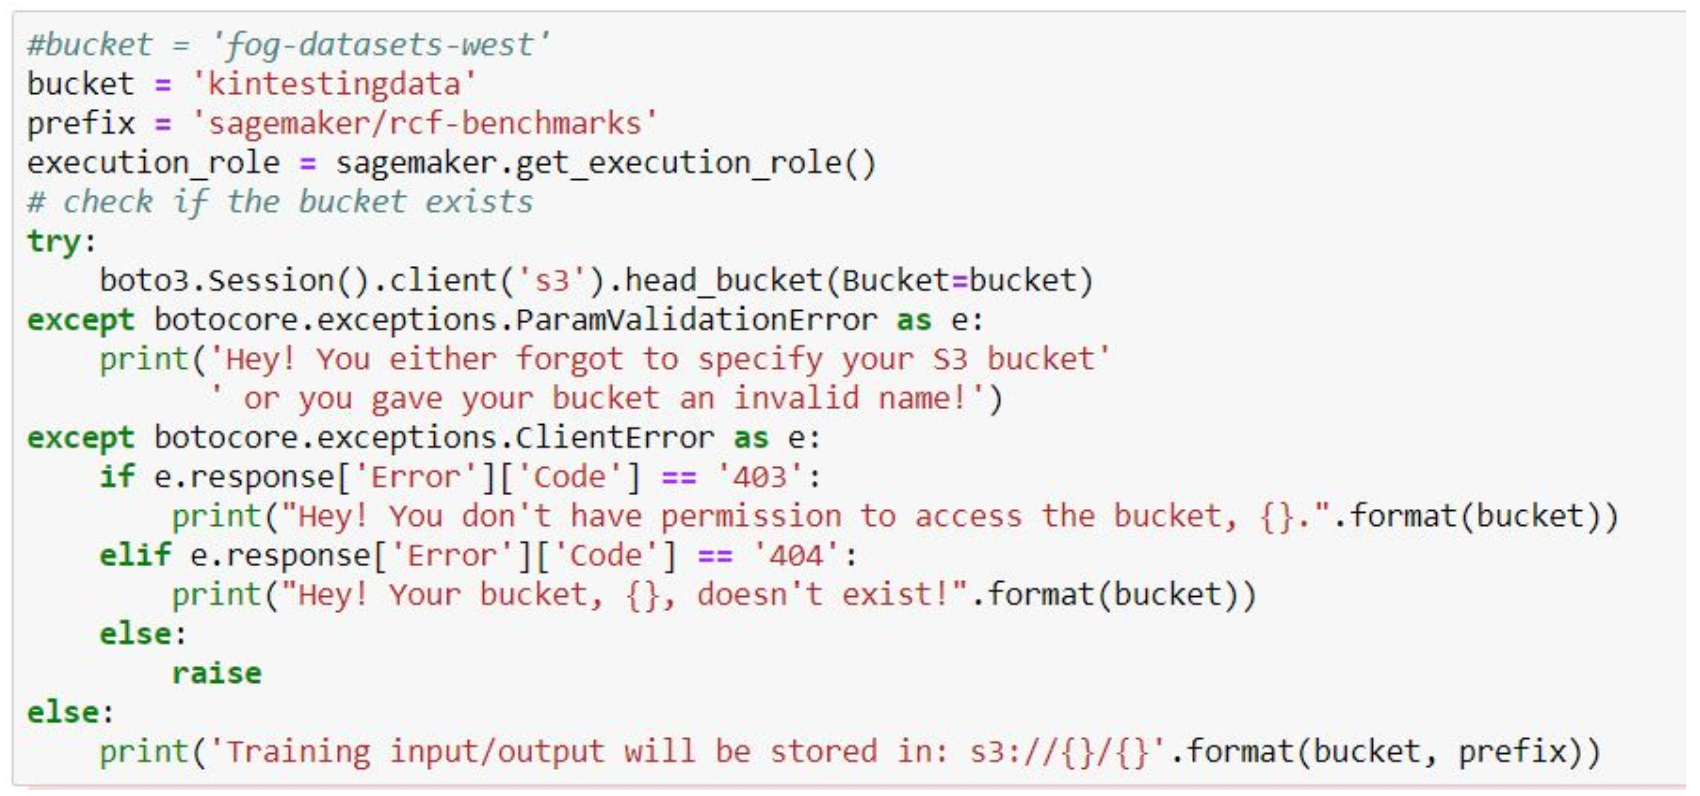
\includegraphics[width=1\textwidth]{images/rcf-data-location.png}
    \caption{Specifications for data location}
    \label{fig:rcf_data_location}
\end{figure}
Next, we configure a SageMaker training job to train the Random Cut Forest (RCF) algorithm on one minute data.

\textbf{Hyperparameters}\\
Particular to a SageMaker RCF training job are the following hyperparameters:
\begin{itemize}
    \item \textit{num\textunderscore samples\textunderscore per\textunderscore tree} - the number of randomly sampled data points sent to each tree. As a general rule, 1/\textit{num\textunderscore samples\textunderscore per\textunderscore tree} should approximate the estimated ratio of anomalies to normal points in the dataset.
    \item \textit{num\textunderscore trees} - the number of trees to create in the forest. Each tree learns a separate model from different samples of data. The full forest model uses the mean predicted anomaly score from each constituent tree.
    \item \textit{feature\textunderscore dim} - the dimension of each data point.
\end{itemize}
Along with these RCF model hyperparameters, we provide additional parameters defining things like the EC2 instance type on which training will run, the S3 bucket containing the data, and the AWS access role. Note that,
\begin{itemize}
    \item Recommended instance type: ml.m4, ml.c4, or ml.c5
    \item Current limitation: The RCF algorithm does not take advantage of GPU hardware.\footnote{ https://docs.aws.amazon.com/sagemaker/latest/dg/randomcutforest.html}\\
\end{itemize}
\begin{figure}[h]
    \centering
    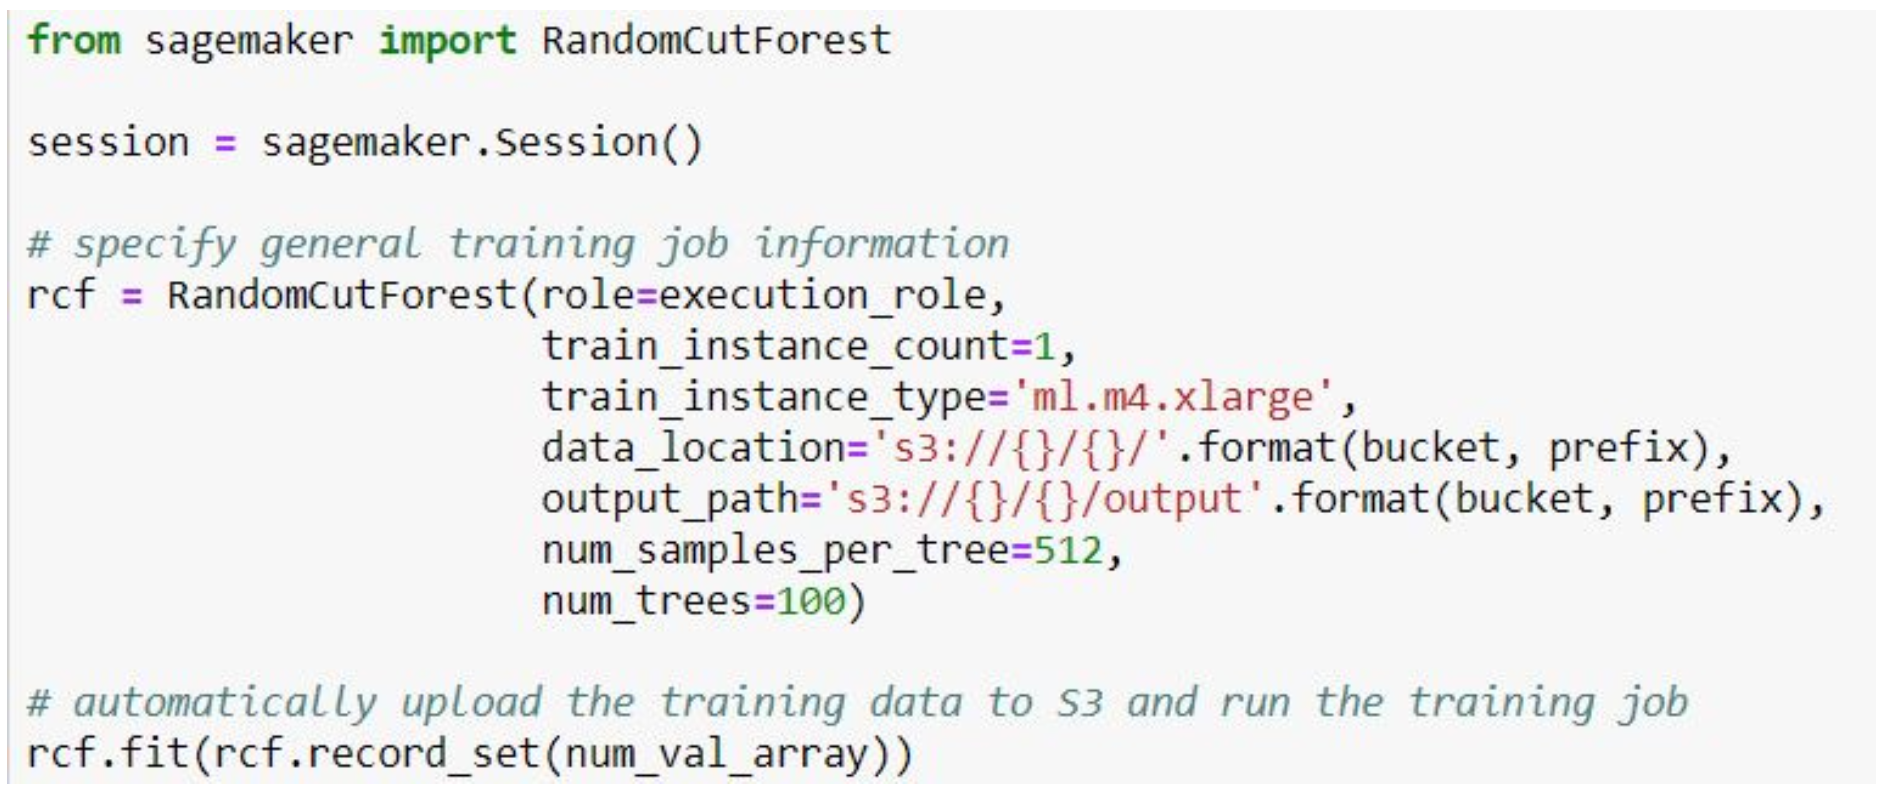
\includegraphics[width=1\textwidth]{images/rcf-model-training.png}
    \caption{RCF Model training}
    \label{fig:rcf_model_training}
\end{figure}
We used SageMaker Python SDK deploy() function from the job to create an inference endpoint. The function has two input parameters:  the instance type and an initial number of instances. 

There are two ways to invoke the trained model:
\begin{itemize}
    \item Right after training in the same notebook, calling a job’s \textit{predict(Test\textunderscore data)} function
    \item From elsewhere(e.g., inside a lambda function), using a function \textit{runtime.invoke\textunderscore endpoint\\(EndpointName, ContentType, Body)}
\end{itemize}
The model outputs an anomaly score for each input data point. It is suggested in a RCF documentation, to compute a value of the anomaly threshold as 3 standard deviations from the mean score. Any value that is beyond the threshold is considered as an anomaly. 
The way to compute the threshold value is subject to change. Depending on business requirements, one can calculate it either once for the whole period of data, or for shorter periods of time, e.g., recompute threshold every day.\\We decided to experiment and calculate the threshold per each day and these results are available below.
The first following plot represents the data, the second one demonstrates testing results. The red plot depicts threshold values that we compute for each day. As we can see, not only high local peaks are detected as anomalies, but also local downfalls and congestions on bottoms are anomaly candidates. 
\begin{figure}[h]
    \centering
    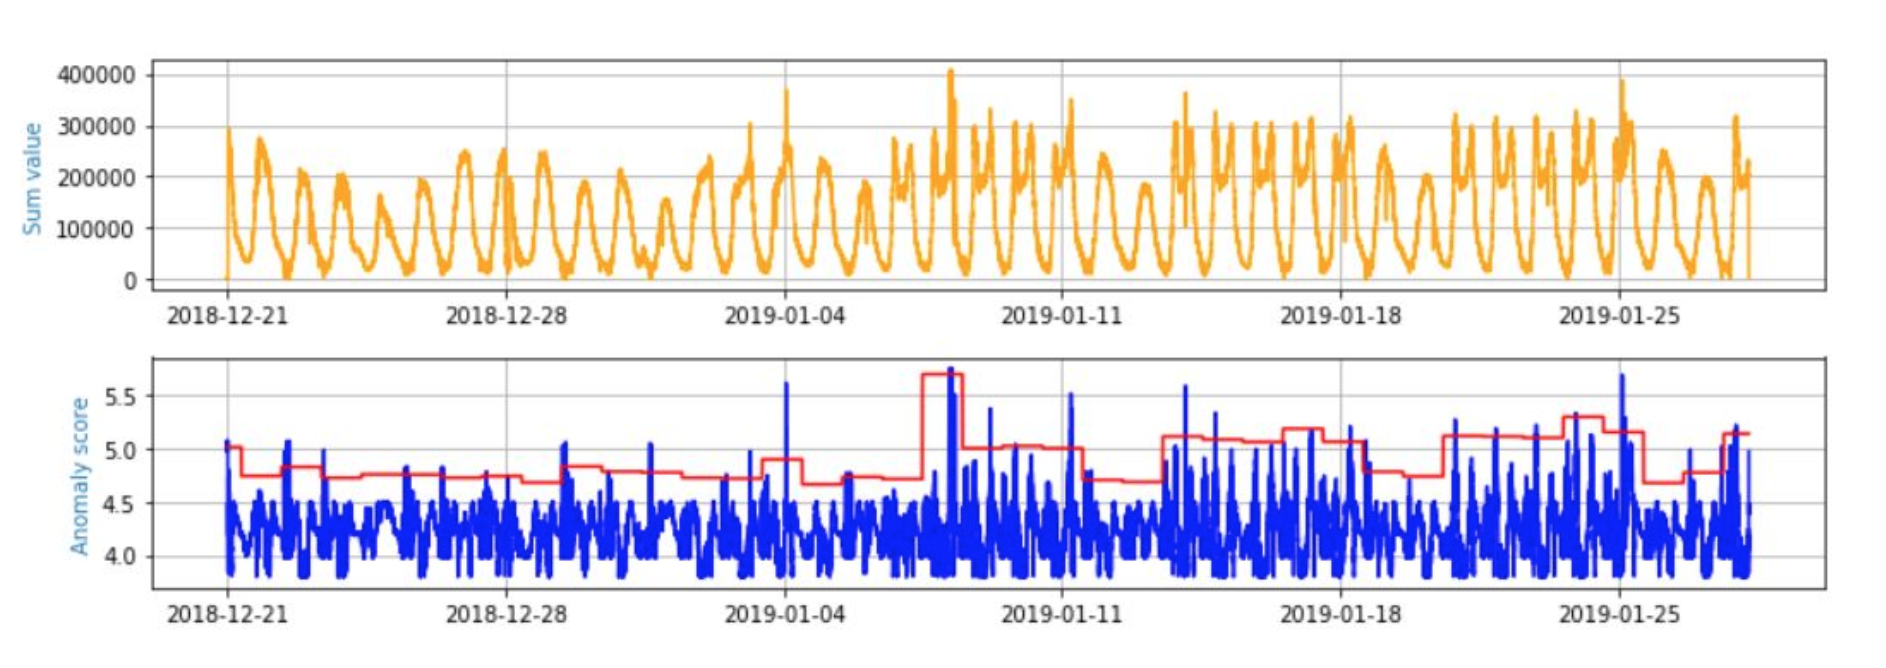
\includegraphics[width=1\textwidth]{images/rcf-results.png}
    \caption{Plotted data, anomaly scores, and anomaly threshold values}
    \label{fig:rcf_results}
\end{figure}
\FloatBarrier



    \FloatBarrier
    
\subsection{Mean Predictor Algorithm}
    %Author: Marius
\textit{Author: Marius Schidlack} \\
\label{mean-predictor}
\paragraph{Motivation}
While sophisticated algorithms like the random cut forest seem to be promising for fitting large amounts of data with complex patterns, they did appear overly complicated for the amount and nature of the data at hand. The data shows a clear weekly periodicity, where the data from one week can hardly be distinguished from another. The only exception is the one week of holidays. In fact, the weeks are so similar, that we can predict the same pattern every week with high confidence. This was the motivation for us to implement a very simple, yet effective machine learning model called the Mean Predictor.

\paragraph{Idea}
The main idea is already contained in the name Mean Predictor. The objective of the Mean Predictor is to calculate the expected week and standard deviation for each point in a week. Accordingly, we can identify outliers by simply checking if the data point lies within the allowed deviation of the expected value. 

Unfortunately, AWS Sagemaker does not offer a Mean Predictor as an Out-Of-The-Box algorithm like the Random Cut Forest. Thus, we implemented it ourselves.

\paragraph{Implementation}

\begin{figure}
    \centering
    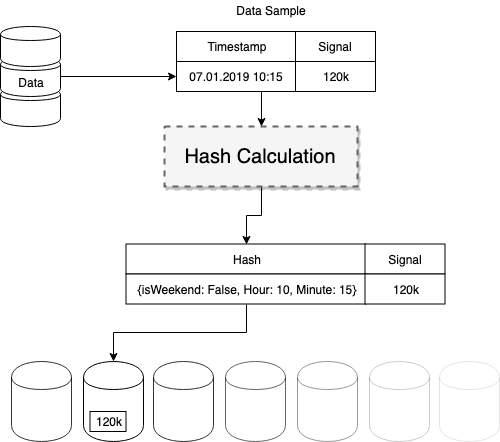
\includegraphics[width=0.6\textwidth]{images/mean_predictor_hashing.png}
    \caption{Hashing process of Mean Predictor Model}
    \label{fig:mean_predictor_hashing}
\end{figure}

For calculating the expected week, we sorted every data point into a bucket that is determined by its \textit{Timestamp}. Each bucket has a hash or index associated with them. After distributing all the data into buckets, we calculate the mean of all the values in one bucket, as well as a measure of standard deviation. This process is visualized in figure \ref{fig:mean_predictor_hashing}.

The hashing function is central to this approach, as we can arbitrarily craft the features that we want our mean predictor to represent. Apart from the weekly periodicity of the data, we also noticed a very predictable daily pattern throughout the working week. Hence we decided to put all working days into one set of buckets and all weekend days into a different set. We did this to ensure a reasonable amount of samples for each bucket. The hashing function currently employed in the mean predictor is shown in  code example \ref{lst:timestamp_hashing}. As more and more data comes in, the function can be adjusted if necessary.

% wrap in minipage so the code doesnt get split to multiple pages
\begin{minipage}{\linewidth}
\begin{lstlisting}[caption={Time stamp hashing function used for Mean Predictor},label={lst:timestamp_hashing}]
def __time_hash(self,t):
       return (t.weekday() < 5,t.hour,t.minute)

\end{lstlisting}
\end{minipage}

As mentioned before, we also require a measure of expectation deviation for determining outliers. The first thing that comes to mind is the standard deviation:

\begin{equation}
\begin{aligned}
\sigma_t = \sqrt{\frac{1}{n}\sum_{i=1}^N (s_t^{(i)} - \mu_t)^2}\\
\end{aligned}
\end{equation}

Where $\mu_t$ denotes the mean value of bucket $t$ and $s_t^{(i)}$ the $i$-th value in this bucket. However, since we square the distance from the mean, the standard deviation weighs outliers much heavier than conform data, which might not be the desired behaviour for the task at hand, because outliers are what we want to detect. Instead one might want to use the average euclidean distance from the mean:
\begin{equation}
\begin{aligned}
\sigma_t = \frac{1}{n}\sum_{i=1}^N \sqrt{(s_t^{(i)} - \mu_t)^2}\
\end{aligned}
\end{equation}
In our case, the choice of deviation measure had little influence on the final results, nevertheless if future training data is noisy and contains a lot of outliers, this might be an option to consider. 

\paragraph{Training and Prediction}
\begin{figure}[h]
    \centering
    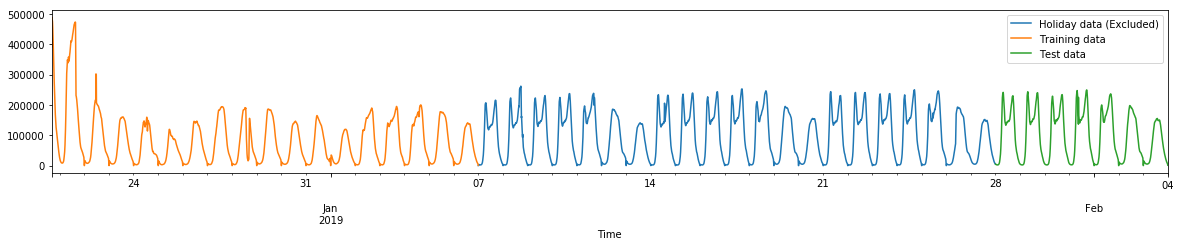
\includegraphics[width=1\textwidth]{images/mean_pred_training_data.png}
    \caption{Train-Test split of data used for the mean predictor}
    \label{fig:mean_predictor_training_data}
\end{figure}
Due to the fact that the Christmas holidays are included in the data, a lot of the provided training data is anomalous and therefore not useful for training a model that is supposed to detect anomalies. Accordingly, we excluded this data from training, leaving us with only three weeks of training data. Alternatively one could also alter the hashing function to give holidays a separate set of buckets. Our train-test split is shown in figure \ref{fig:mean_predictor_training_data}.

\begin{figure}
    \centering
    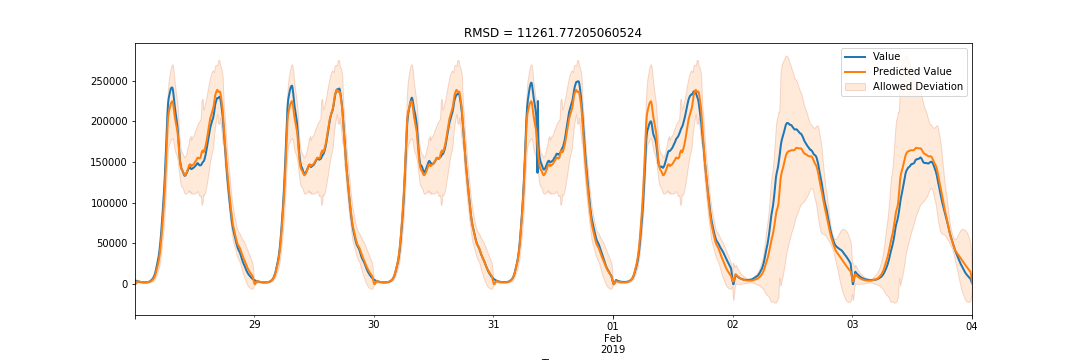
\includegraphics[width=1\textwidth]{images/mean_pred_test.png}
    \caption{One week prediction of Mean Predictor model}
    \label{fig:mean_predictor_prediction}
\end{figure}

Once we have expected value and deviation for each bucket, making predictions is trivial. The model simply takes a time interval and calculates the hash for each timestamp within that interval. We obtain the prediction by simply looking up the expected value and deviation in our table. Figure \ref{fig:mean_predictor_prediction} depicts a prediction for the week starting at the 28th of January 2019 (test set) and compares it to the ground truth. For this test data, the prediction is highly accurate and the true values never leave the confidence interval. The RMSE \textit{(Root Mean Squared Error)} of the prediction lies around 11,261. Further investigation is needed to accurately assess the outlier detection performance, since we were lacking test data that contains real outliers. For the time being, by looking at the confidence interval, we can see that sudden spikes or lows in the timeseries could easily be identified as anomalies.
\pagebreak

\paragraph{Deployment as Sagemaker Endpoint}
In order to use our model in the Cloud, we deployed it as an AWS Sagemaker Endpoint. In the following we describe the technical details related to this task. The endpoint was implemented along the lines of a tutorial provided by AWS \footnote{\url{https://github.com/awslabs/amazon-sagemaker-examples/blob/master/advanced_functionality/scikit_bring_your_own/scikit_bring_your_own.ipynb}}.

Sagemaker Models are deployed from docker images. Hence, we defined a docker file that encapsulates the model into a container. The container image is then built and uploaded to AWS \textit{Elastic Container Registry} (ECR) with the \textit{build\_and\_push.sh} script. The \textit{train\_deploy.py} script provides a convenient command line interface for spinning up a Sagemaker endpoint using the previously uploaded container image. This script can also be embedded into a terraform pipeline.
The model requires only one hyperparameter: The granularity or \textit{frequency} with which it should make the timeseries predictions. Furthermore it needs a path to the training data located in a S3 Bucket.

At its core, the Sagemaker endpoint is nothing but a REST-API that takes training jobs and prediction requests and forwards it to the Mean Predictor. Once deployed, the endpoint takes prediction requests in the following JSON format:

\begin{lstlisting}
{
    "start": "YYYY-MM-DD HH:MM:00",
    "end": YYYY-MM-DD HH:MM:00
}
\end{lstlisting}

It will respond with a time series prediction within the \textit{start}-\textit{end} interval, depending on the aforementioned \textit{frequency}. The response is delivered in the following CSV-Format:

\begin{center}
    \begin{tabular}{ | l | l | l |}
    \hline
    Timestamp & Value & Std \\ \hline
    2019-01-05 10:15:00 & 100 & 7 \\ \hline
    2019-01-05 10:20:00 & 96 & 13 \\ \hline
    2019-01-05 10:25:00 & 112 & 8 \\ \hline
    \dots & \dots & \dots \\
    \hline
    \end{tabular}
\end{center}

Similar to the Random Cut Forest, the model will not do outlier detection by itself, but rather provide the user with the necessary information to do so. In order to detect an outlier, one must simply check if a specific data point lies within the bounds of allowed deviation at that time. The user can arbitrarily scale the allowed deviation to their requirements. Such functionality is easily implemented within an AWS Lambda function, which allows seamless integration of the model into the Cloud Architecture. Furthermore, it allows to use the same model for anomaly detection and prediction at the same time.

\paragraph{Conclusion}
The Mean Predictor is of course a very minimalistic approach: in its current state, we can only incorporate a single source of information, it is not able to leverage additional data, e.g. weather data to improve its prediction. The model is not able to learn features of the time series by itself. As the prediction will resemble a regular working week every time, the model is of little use during holiday periods, however, once enough data is gathered, the hashing function can be manually adjusted to differentiate between holiday and working weeks. With the small amounts of training data and the selected test set, the prediction of the Mean Predictor vastly outperforms the other, more complex, Machine Learning models that we examined with an RMSE of just 11,261.

\subsection{Real time anomaly detection with Kinesis}
    \label{sec:real_time_anomaly_detection}
\textit{Author: Clemens Peters} \\
\subsubsection{Motivation}
This approach is inspired by a Medium blog post\cite{MEDIUM}.
Note that this approach is entirely different to the aforementioned ones, and does \textbf{not} build on the architecture shown in figure \ref{fig:architecture}. Instead, a different architecture is incorporated which will also be described in this section.
The goal of the approach is to move the anomaly detection closer to a real-time setup. This means to continuously process the most recent data instead of analyzing data from the previous month or year to find anomalies. To give some more motivation about why this is actually an important issue, here is a quote from a job description from Netflix\cite{NETFLIX}:
\begin{displayquote}
    "Netflix Operational Insight Team is the team responsible for building common infrastructure to collect, transport, aggregate, process and visualize operational metrics. We build powerful systems to allow everyone at Netflix visibility into the state of our environment at both a macro and micro level."
\end{displayquote}
The fact that a leading and modern company like Netflix builds a whole team just dedicated to checking and visualizing the current system state in real time, underlines how important it is to know at every moment how your environment performs.\\
AWS Kinesis is a very suitable tool for this problem for multiple reasons. First of all, Kinesis is designed to process streaming data. This means we can ingest real-time data which is a perfect fit for our given VPC Flowlog data. Second Kinesis comes with Kinesis Data Analytics already built in. Amazon Kinesis Data Analytics offers easy ways to analyze streaming data, gain actionable insights, and respond to business needs in real time. In addition to that there is a SQL function called “Random cut forest with explanation” which is described by AWS as follows:
\begin{displayquote}
    Computes an anomaly score and explains it for each record in your data stream. The anomaly score for a record indicates how different it is from the trends that have recently been observed for your stream. The function also returns an attribution score for each column in a record, based on how anomalous the data in that column is. For each record, the sum of the attribution scores of all columns is equal to the anomaly score. \cite{awsRcf}
\end{displayquote}

\subsubsection{Architecture}
Given this prior knowledge, we will now dive further into the system setup.
First let us get an overview of the system as it was implemented during the project phase:
\begin{figure}
    \centering
    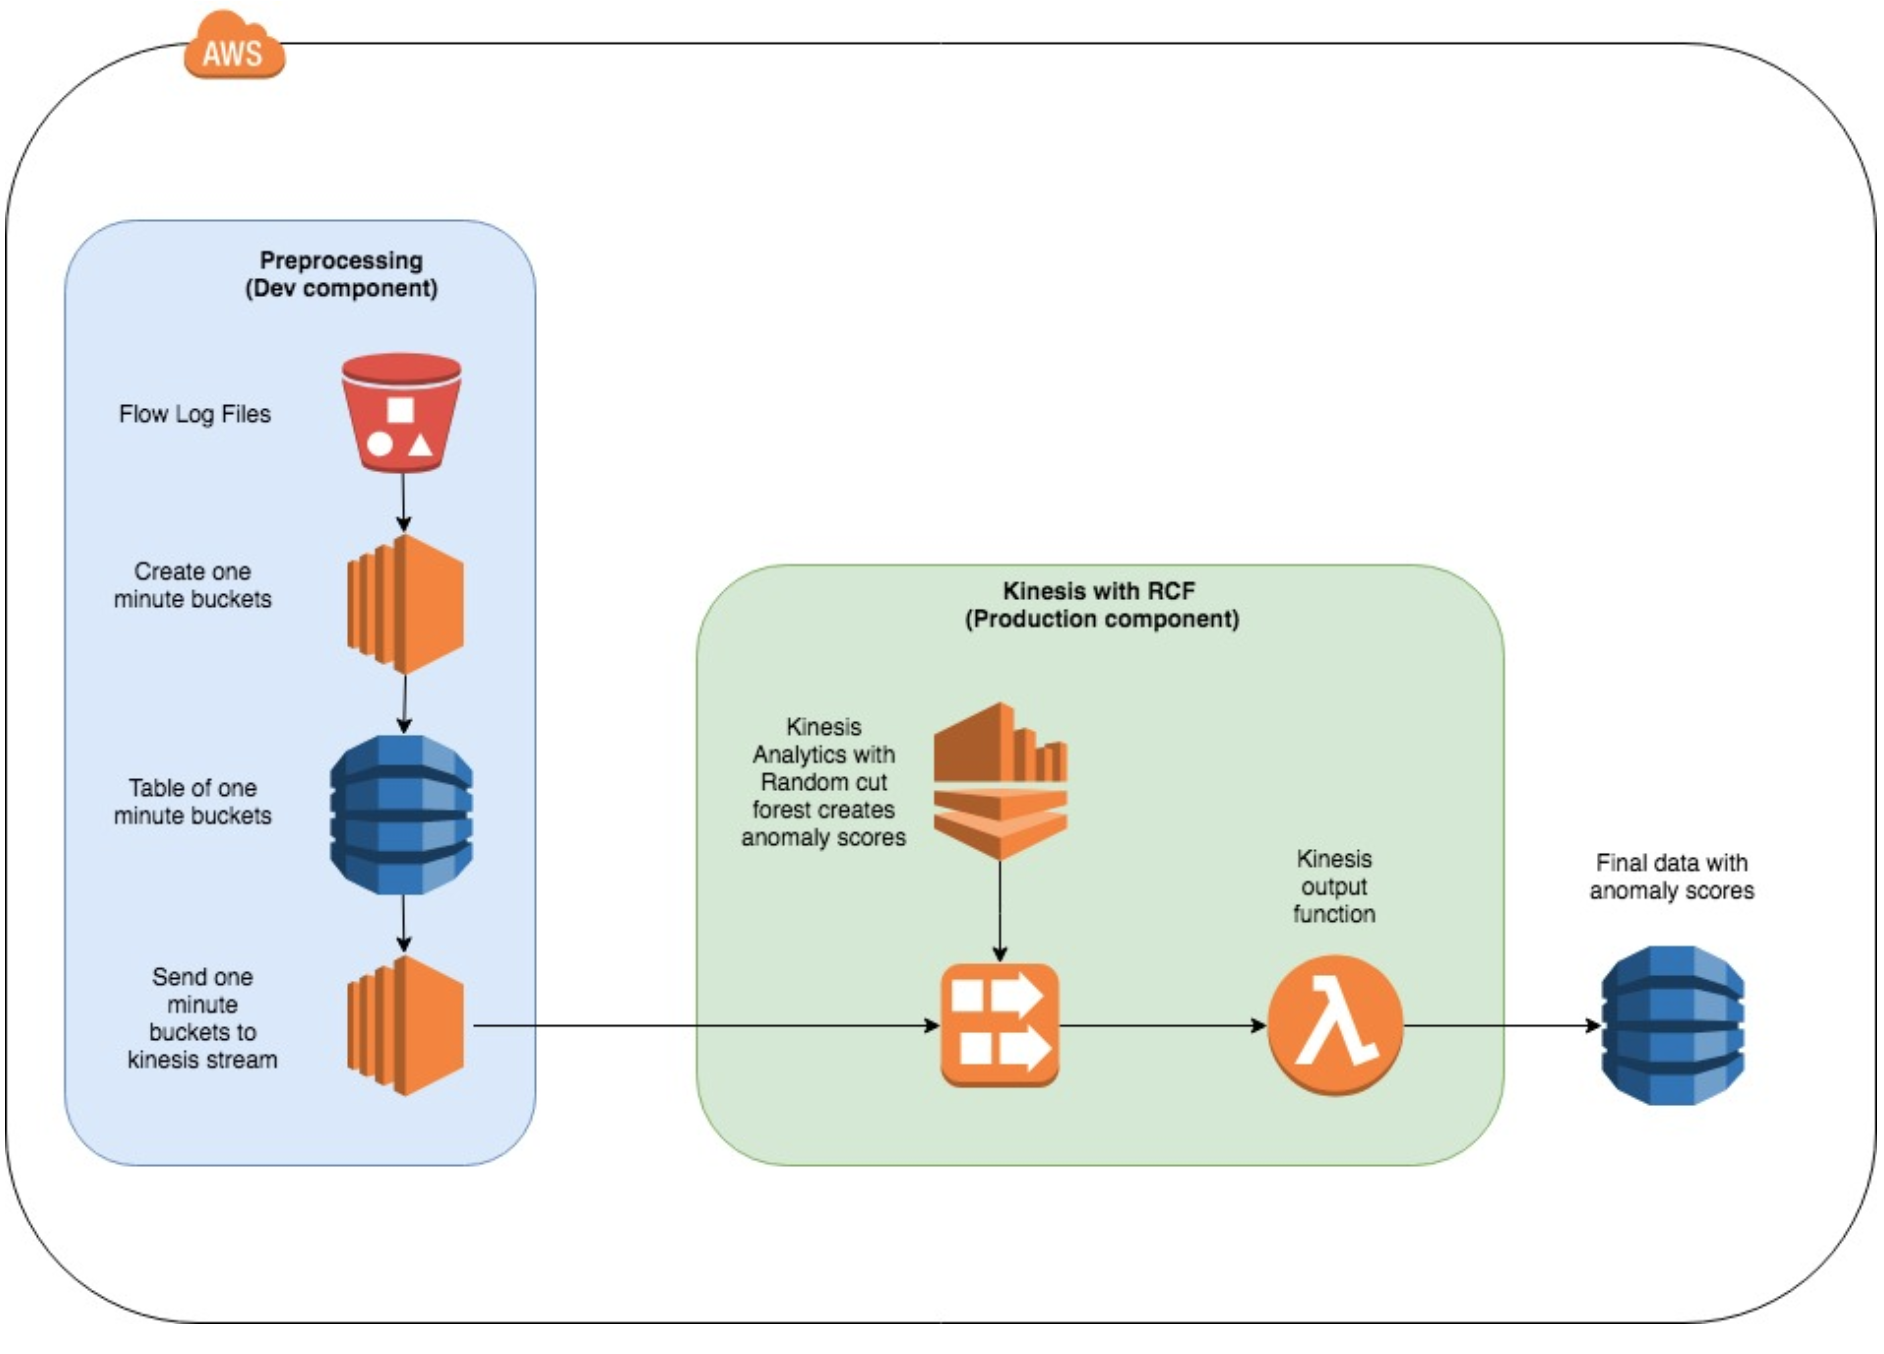
\includegraphics[width=1\textwidth]{images/medium-kinesis-setup.png}
    \caption{Medium Kinesis Random Cut Forest Setup}
    \label{fig:medium_kinesis_setup}
\end{figure}
\FloatBarrier
To start with, it should be noted that all the preprocessing components on the left (blue area in figure \ref{fig:medium_kinesis_setup}) would not be part of a production system. In a production system we would have a continuous stream of VPC Flowlogs which needs to be handled and preprocessed, whereas in the project setup we had all the Flowlogs data from the past in a S3 bucket. 

\subsubsection{Preprocessing components (blue area in figure \ref{fig:medium_kinesis_setup})}
In the following section we will look at the preprocessing setup in detail, keeping in mind that this is not created to run in production.

\textit{\underline{S3: Flowlogs Files}}\break
All the Flowlogs data provided by BMW lies in an S3 bucket called \textit{fog-bigdata-bmw-data}. As mentioned in section \pageref{sec:fixed_data}, there are two types of data: first the Metrics, which already contain summaries about how many requests were made to the system during a certain time interval. Another issue here was, that the time intervals are of different size (sometimes five minutes, sometimes four or six or something similar). Of course this is not a good basis to run our anomaly detection, because we cannot know what value we expect (since the size of the intervals are different). Therefore the second type of data is more suitable, namely the raw VPC Flowlogs. However, we want to look at how many requests are made to our system per minute and thus we need to do some preprocessing.

\textit{\underline{EC2: create one minute buckets}}\break
At this point, the first script with the name \textit{createOneMinuteBuckets.py} comes in. This script is executed on an EC2 instance and reads all the flow log records from the S3 bucket. It creates one-minute buckets from the Flowlogs, so that we know for every one minute time interval how many requests were made to the system. 

\textit{\underline{DynamoDB: table of one minute buckets}}\break
The information about these one minute buckets is then written into a DynamoDB table (called \verb|medium_bmw_data_to_kinesis|). For the sake of this project the data from the Kinesis table was then exported to a CSV file and the information about the weekdays was added (currently done in Excel). This means that for every one minute bucket we know the hour and the minute and also on which weekday it was recorded. This might be relevant because the expected number of request at 8am on a Sunday can be very different than 8am on a Monday, especially because the requests come from driving cars.  Of course this step will not be part of a production system (as mentioned before).

\textit{\underline{EC2: send one minute buckets to Kinesis stream}}\break
The next script is called \textit{generateAnomalyScores.py}. The script and the final CSV file is uploaded to an EC2 instance again. The script takes the data from this CSV file and sends it to the Kinesis stream called \textit{medium\textunderscore VPCFlowLogs}. An alternative setup could be to read the data directly from DynamoDB and add the information about the weekday in the python script (instead of using CSV and Excel).\\
This is where the preprocessing part (which would look different in a production system) ends and where the production component (green area in figure \ref{fig:medium_kinesis_setup}) comes into play.\\

\subsubsection{Production component (green area in figure \ref{fig:medium_kinesis_setup})}
In this section we assume that we already have all the data we need in the right format. This is the part of the system where the anomaly detection happens. This part of the setup can be used in a production environment in the same or in a similar way. All the preprocessing is done and the data is already fed into the our Kinesis stream.
\begin{figure}
    \centering
    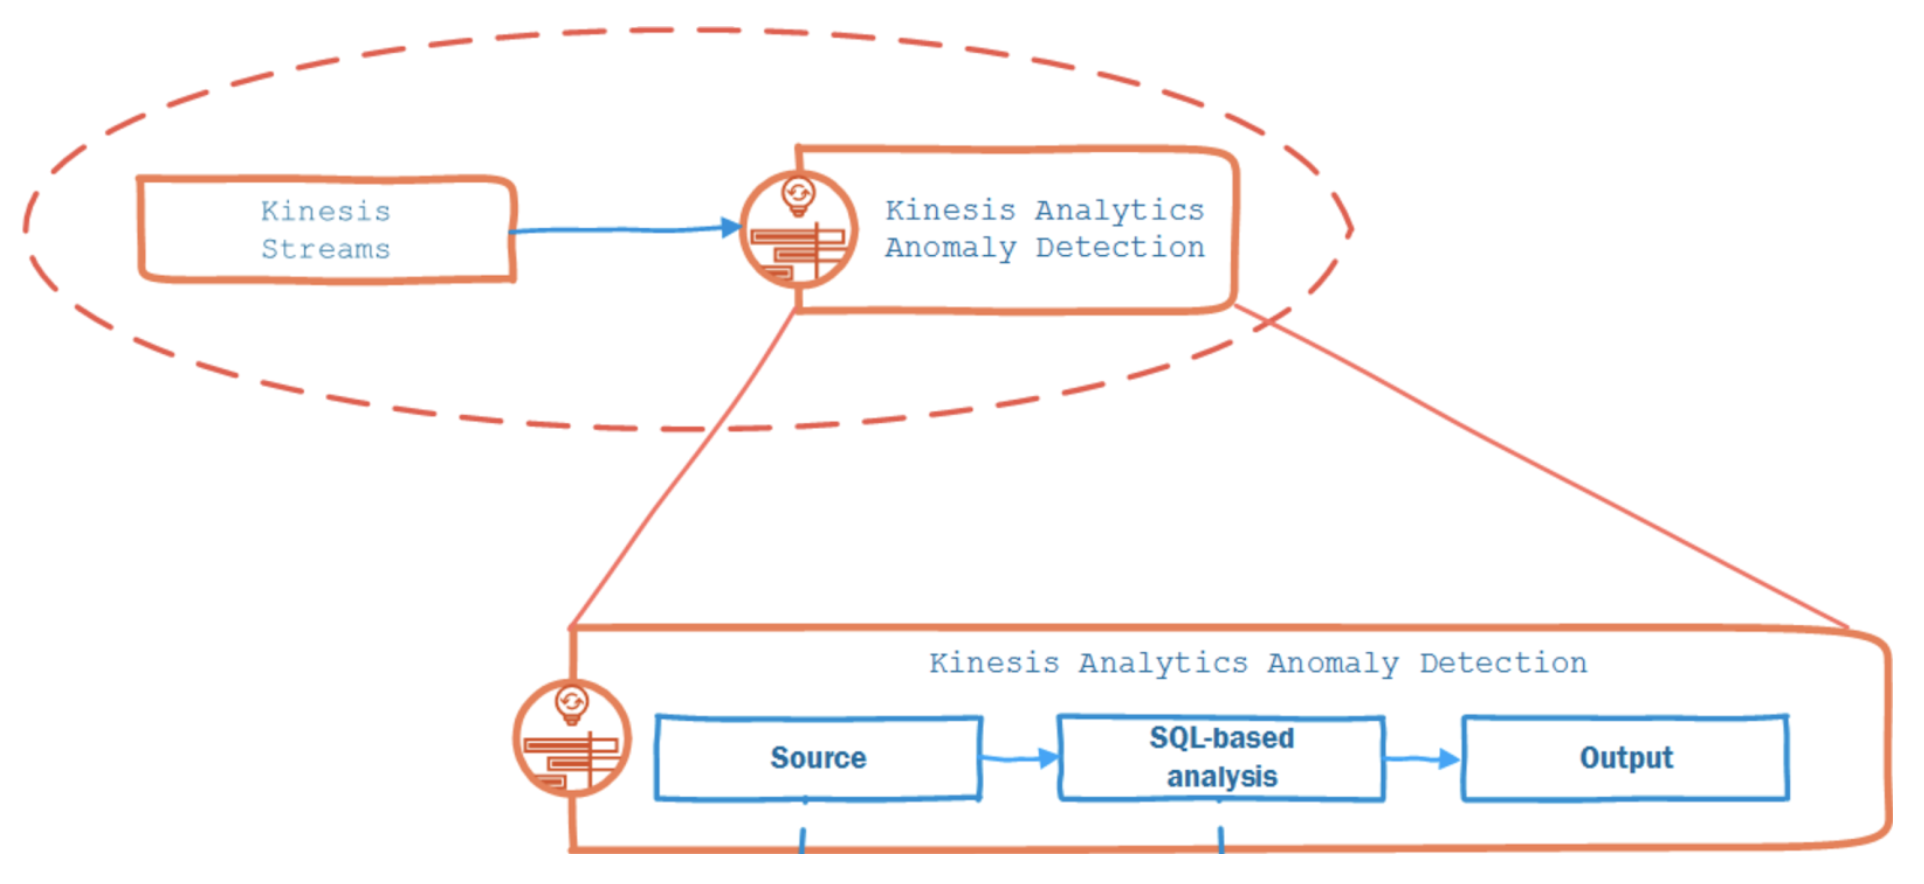
\includegraphics[width=1\textwidth]{images/kinesis-rcf.png}
    \captionsource{Kinesis Data Analytics with RCF}{\\\scriptsize{Source: https://medium.com/@devfire/real-time-anomaly-detection-in-vpc-flow-logs-part-5-anomaly-detection-d1fc9b61baf8}}
    \label{fig:medium_kinesis_data_analytics_rcf}
\end{figure}
\FloatBarrier
The Kinesis stream has a Kinesis Data Analytics application which sends the data to random cut forest where the anomaly scores are created. This is the SQL code for the real time analytics:
\begin{figure}
    \centering
    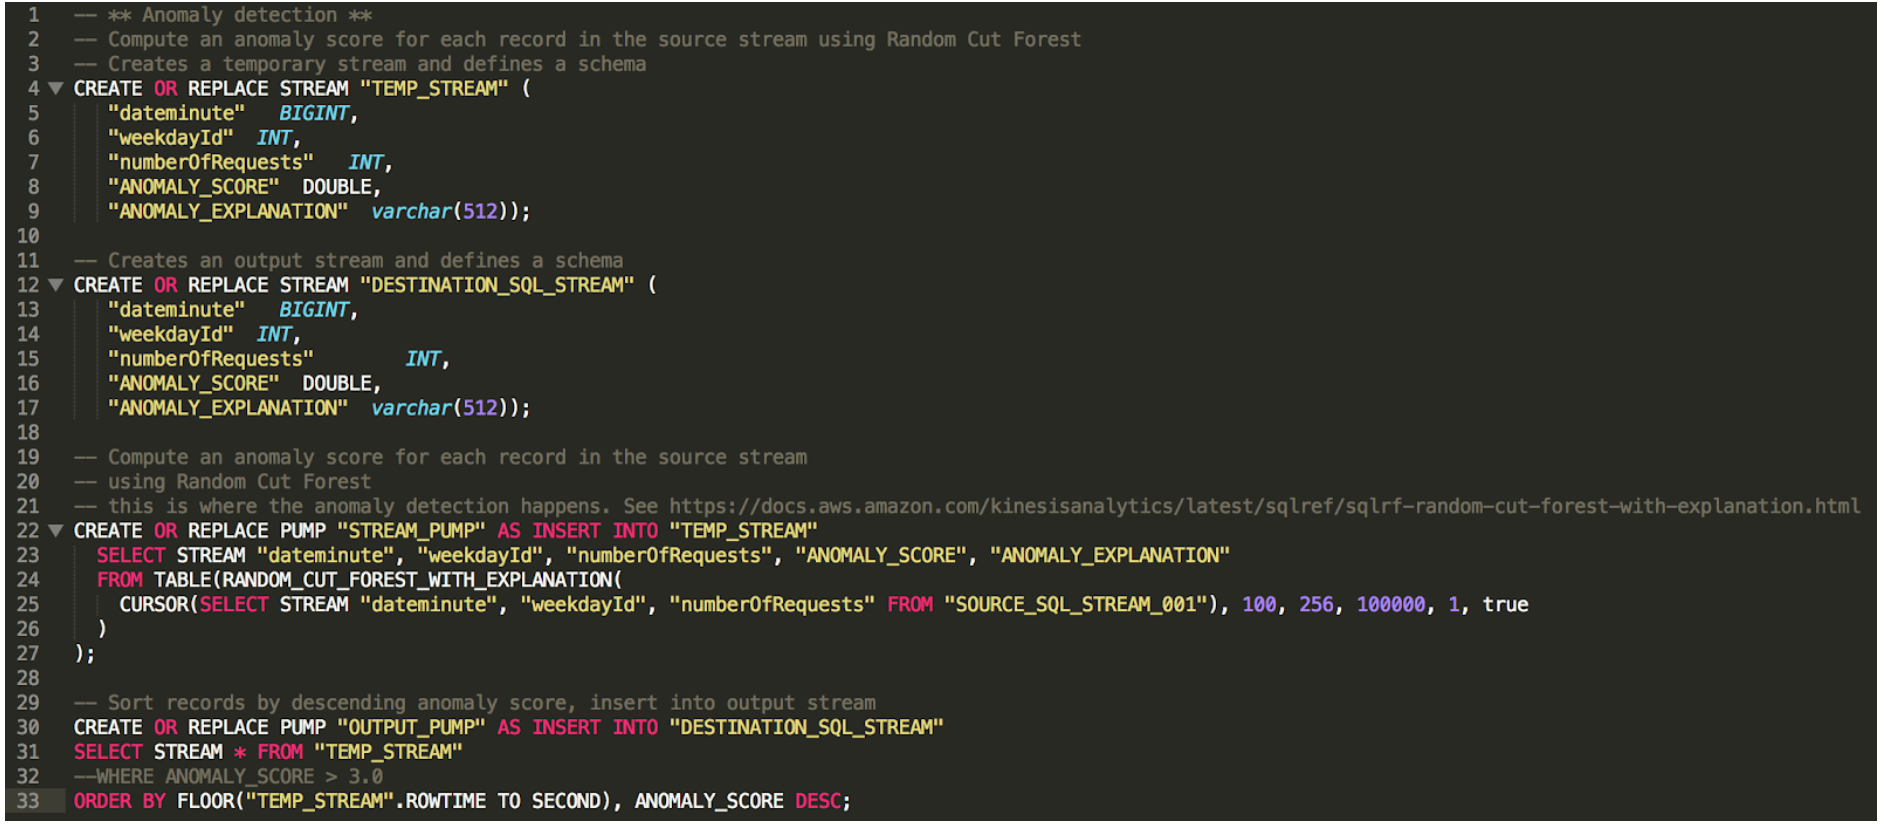
\includegraphics[width=1\textwidth]{images/sql-analytics.png}
    \captionsource{SQL code for real time analytics}{\\\scriptsize{Source: https://medium.com/@devfire/real-time-anomaly-detection-in-vpc-flow-logs-part-5-anomaly-detection-d1fc9b61baf8}}
    \label{fig:medium_sql_analytics}
\end{figure}
\FloatBarrier
As we can see from the comment in line 32 it would be possible to already define a threshold here. This would then mean, that only anomaly scores which are higher than that specified threshold are sent to the output stream. However, it is recommended to implement this threshold in the output lambda function, to keep the threshold logic separate from the creation of the anomaly scores. Furthermore it is a lot easier to version and backup the lambda function in case the threshold is changed over time than to maintain different versions of the SQL code in the Kinesis Data Analytics part.

\textit{\underline{Lambda: Kinesis output function}}\break
The output of the Kinesis stream is sent to the Lambda function\\ \verb|medium_bmw_kinesis_to_dynamodb_2|. 
This Lambda function just stores the results to another DynamoDB called \verb|kinesis_bmw_anomaly_scores|. Obviously this last database table was just for the purpose of the project phase to collect all the anomaly scores and visualize them in a graph but it is not needed in a production setup (as indicated in the system architecture). Instead, in a production system this output function should contain the threshold for the anomaly score and then send a message or trigger a phone call if the threshold is exceeded.

\subsubsection{Results}
\begin{figure}[h]
    \centering
    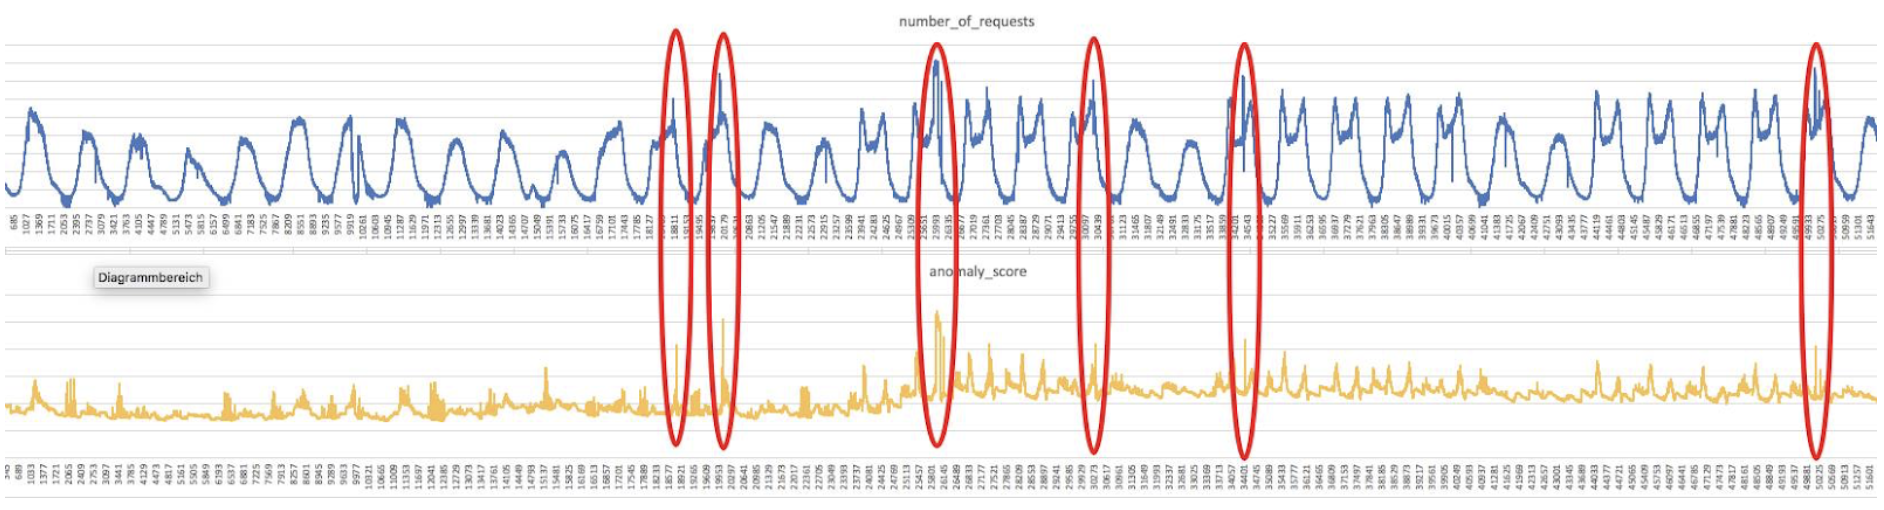
\includegraphics[width=1\textwidth]{images/kinesis-results.png}
    \caption{Visualisation of Kinesis Analytics Results}
    \label{fig:medium_kinesis_results}
\end{figure}
\FloatBarrier
The blue graph at the top of figure \ref{fig:medium_kinesis_results} shows the requests to the the system per minute (from the one minute buckets). The orange graph at the bottom of figure \ref{fig:medium_kinesis_results} visualizes the anomaly score at that time. This means if we see an unexpected high peak or unexpected low drop in the first graph (number of requests per minute), in both cases we would expect a peak in the second graph (the anomaly scores). All in all this example does not show a perfect result (since we would expect our anomaly scores to be consistently low when there is no anomaly), however we have to take into account that this particular data set show the requests from December 21, 2018 until January 28, 2019, which means that it starts with the Christmas holidays. As we know, holidays to not coincide with the normal pattern of five working days followed by two weekend days which we see towards the end.\\ Furthermore, this is a series of 54,689 one minute buckets which is not a very long series to train on. Despite these factors of having limited and atypical data the high spikes in the anomaly scores (highlighted by the red ellipses) indicate that the approach in general is quite promising and that it can already detect anomalies.

\subsubsection{Future work}
The presented results are retrieved from feeding the data into the Random Cut Forest in the following format: date-minute data, the weekday ID (as an integer) and number of requests.
To refine the system further it might be interesting to try different combinations of these three input variables to see which combination gives the best results. This way it could be determined if it decreases the performance if we leave out the information about the weekday completely for example.

\subsubsection{Implementation guide (Kinesis Random Cut Forest)} 
This can be found in the appendix of this report (Appendix \ref{appendix-medium}) or online at \url{https://gist.github.com/clemenspeters/8e9025e3bd71e9087df154fb06f96328}